\section{Task: Open a Database}
\label{sec:task_open_database}

This task allows creating new databases, or managing and accessing existing ones. This task can not be run, but is performed using the 'Open' button (as indicated by the inactive 'Run Current Task' button).

\begin{figure}[H]
  \hspace*{-2.5cm}
    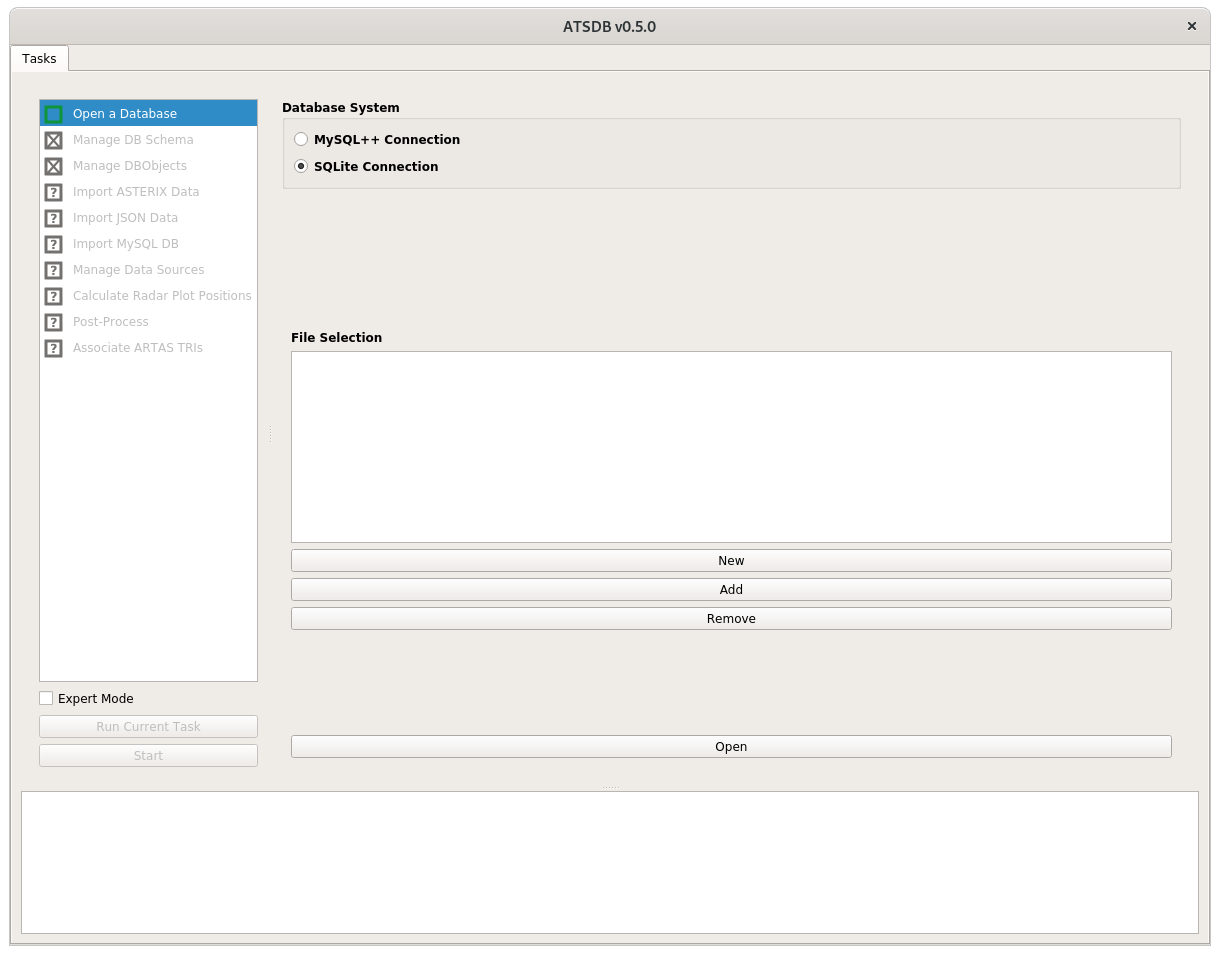
\includegraphics[width=19cm]{../screenshots/task_open_database.png}
  \caption{Task: Open a database}
\end{figure}

Two options exist: Either a MySQL++ connection is used (MySQL or MariaDB server needed) or an SQLite3 database file container is used (no additional setup needed).

\subsection{Opening a SQLite3 File Container}
\label{sec:sqlite_open}
For opening a file container, three actions are available:

\begin{itemize}  
\item New: Creates a new (empty) SQLite3 container and adds it to the 'File Selection' list
\item Add: Adds an existing  SQLite3 container and adds it to the 'File Selection' list
\item Remove: Removes an entry from the 'File Selection' list
\end{itemize}

After selection of the wanted database container, the 'Open' button can be used for opening the database container.

\begin{figure}[H]
  \center
    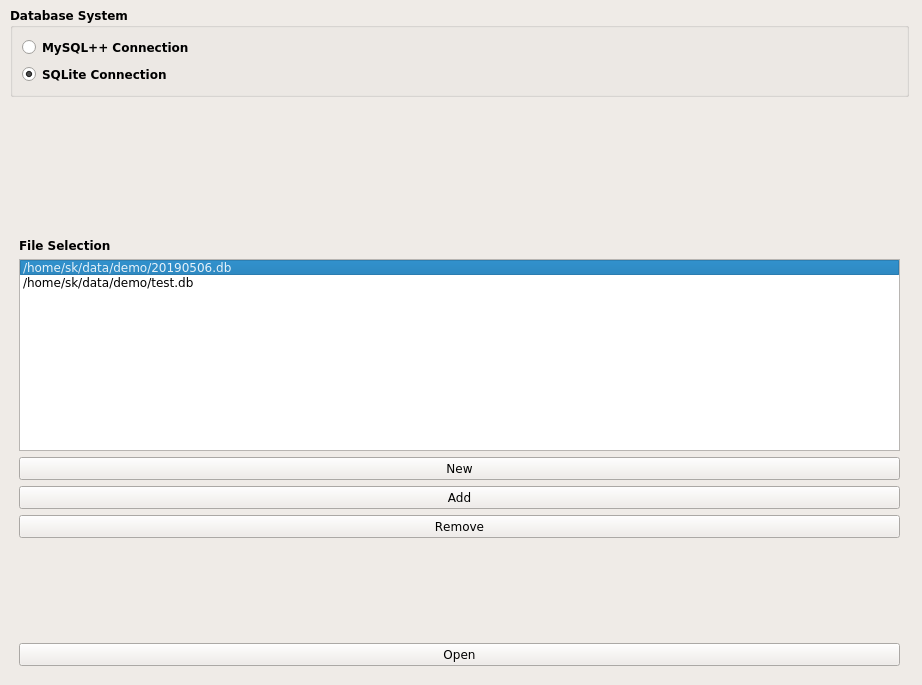
\includegraphics[width=16cm,frame]{../screenshots/sqlite3_open.png}
  \caption{Opening a SQLite3 file container}
  \label{fig:sqlite3_open}
\end{figure} 


\subsection{Connecting to a MySQL Server}
\label{sec:mysql_connect}

\begin{figure}[H]
  \center
    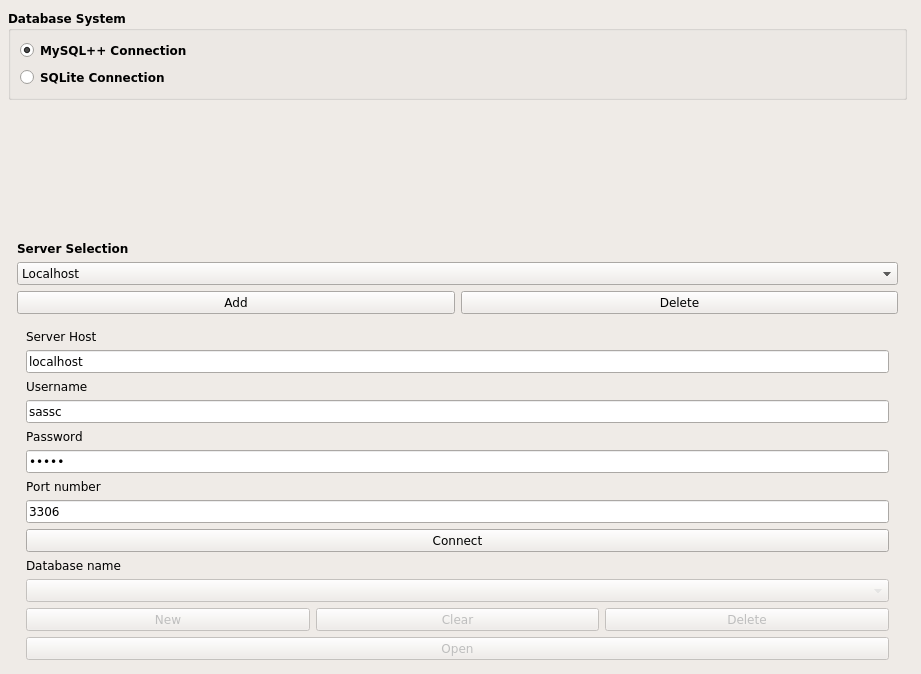
\includegraphics[width=16cm,frame]{../screenshots/mysql_server_selection.png}
  \caption{Connecting to a MySQL server}
  \label{fig:mysql_connect}
\end{figure}

Several MySQL servers can be defined, each one has a specific set of parameters. To add a new server, press the 'Add' button and enter a unique server name. To select the currently used server, use the dropdown menu. To delete the currently used server, press the 'Delete' button.

For connecting to a MySQL server, several parameters have to be entered:

\begin{table}[H]
  \center
  \begin{tabular}{ | l | l | l |}
    \hline
    \textbf{Parameter} & \textbf{Description} & \textbf{Example Values} \\ \hline
    Server Host & Network identifier of server & 'localhost', '10.0.0.123' \\ \hline
    Username & MySQL user name & 'sassc', 'root' \\ \hline
    Password & MySQL user password & 'sassc', '' \\ \hline
    Port Number & MySQL server port & '3306' \\
    \hline
  \end{tabular}
  \caption{MySQL server parameters}
\end{table}

To connect to a defined MySQL server, press the 'Connect' button.\\

\paragraph{Access to SASS-C MySQL Servers}

Please note that it is not recommended to use SASS-C databases on which actual performance evaluations are to be performed. \\
Using ATSDB, database operations can be performed which might impede results later obtained by using SASS-C. For this reason, it is recommended to either clone an evaluation or use one on which no later SASS-C evaluations are performed.

If a remote server is used, e.g. a SASS-C workstation, remote access might be prohibited, which will result in an access permissions error during connecting. To resolve this, (generally) remote access can be enabled in the servers MySQL configuration. As a superuser, edit the file 'my.cnf', which is commonly found under '/etc/mysql/my.cnf'. 

Find the line that states:
\begin{cverbatim}
bind-address = 127.0.0.1
\end{cverbatim}

Change the line to:

\begin{cverbatim}
#bind-address = 127.0.0.1
\end{cverbatim}

Then, restart the MySQL server using one the following commands:

\begin{cverbatim}
/etc/init.d/mysqld restart

#OR, depending on your distribution
service mysql restart
\end{cverbatim}

Then, to allow access to the databases, log into a MySQL client on the server as root and execute the following commands:

\begin{cverbatim}
# log in as root, must be done as superuser
mysql -u root

# grant access rights for your MySQL user, 
# e.g. 'sass', from the your local IP address, 
# e.g. '192.168.0.104', using your password, e.g. 'sassc'
GRANT ALL ON *.* to 'sassc'@'192.168.0.104' IDENTIFIED BY 'sassc';

# set access rights
FLUSH PRIVILEGES;

# exit the MySQL client
exit
\end{cverbatim}

After executing these steps once, remote access to this MySQL server from the specified IP address is enabled.

\paragraph{Firewall}

It might also be the case that your installation of SASS-C has an enabled firewall. If that is the case, access to be MySQL ports must be enabled.

\begin{figure}[H]
  \center
    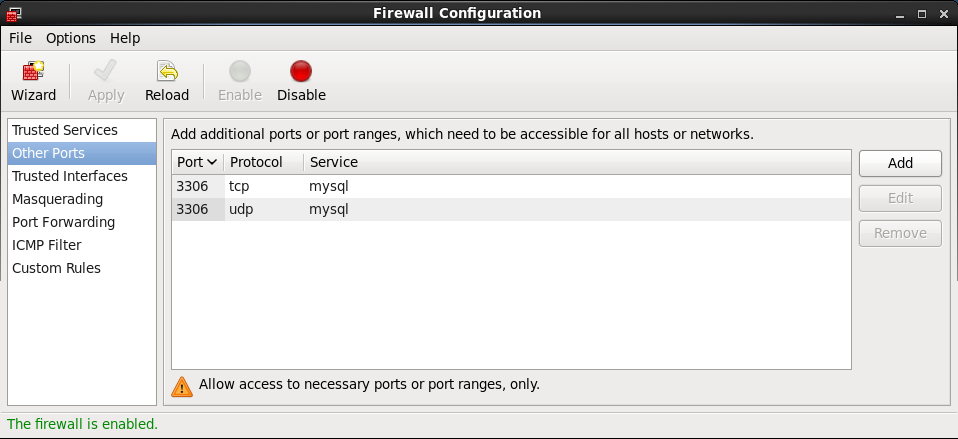
\includegraphics[width=15cm,frame]{../screenshots/centos_firewall.png}
  \caption{CentOS MySQL Server firewall example}
\end{figure}

\paragraph{Error Messages}

If a wrong database name or IP address is used, error messages can be e.g. \\

\begin{figure}[H]
  \center
    \includegraphics[width=9cm,frame]{../screenshots/mysql_connect_error.png}
  \caption{MySQL Server not found error}
\end{figure}

 or 

\begin{figure}[H]
  \center
    \includegraphics[width=9cm,frame]{../screenshots/mysql_user_error.png}
  \caption{MySQL user incorrect error}
\end{figure}

If such an error occurs, correcting the server host name and or user/password should solve the problem. 


\subsection{Opening a MySQL Database}
\label{sec:mysql_open_db}

After successful connection, all existing databases in the server are shown in the 'Database name' drop-down menu. The last used one is selected automatically.

\begin{figure}[H]
  \center
    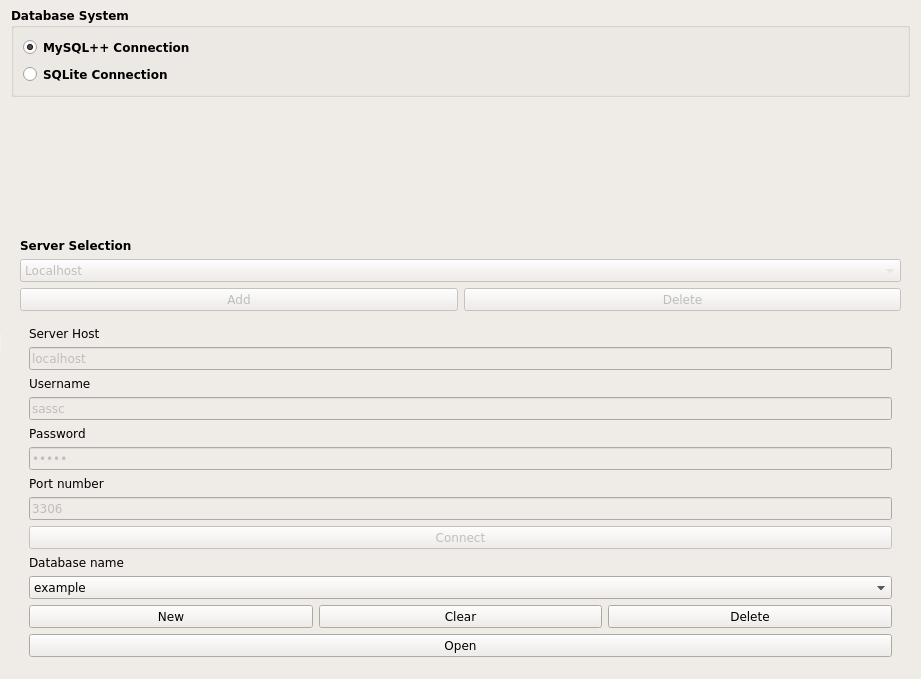
\includegraphics[width=16cm,frame]{../screenshots/mysql_database_selection.png}
  \caption{Selecting a MySQL database.}
  \label{fig:mysql_db_select}
\end{figure}

Several actions are available:

\begin{itemize}  
\item Drop-down selection: Selects the current database
\item New button: Allows creation of a new database
\item Clear button: Deletes all data with current database (after confirmation)
\item Delete button: Deletes current database (after confirmation)
\item Open button: Opens the current database
\end{itemize} 
